\chapter{Decizii arhitecturale}

\section{Ecosistemul Google Cloud}

\subsection{Alegerea platformei agentului}

Comparând Dialogflow cu alte servicii de agenți conversaționali, există mai multe caracteristici care îl diferențiază și îl recomandă pentru utilizarea în sectorul bancar.

Dialogflow, deținut de Google, este o platformă avansată pentru dezvoltarea de aplicații de conversație, care folosește tehnologia AI pentru a interpreta intențiile și contextul utilizatorului \cite{google_dialogflow}. Aceasta oferă o gamă largă de funcționalități, inclusiv integrarea cu diverse platforme de mesagerie, asistenți virtuali și alte servicii Google, cum ar fi Google Cloud Functions.

La rândul lor, serviciile alternative, cum ar fi IBM Watson, Amazon Lex și Microsoft Luis, prezintă și ele avantaje. IBM Watson se remarcă prin puterea sa de a învăța în mod continuu și de a se adapta la diverse contexte de utilizare \cite{ibm_watson}. Amazon Lex beneficiază de integrarea nativă cu ecosistemul Amazon Web Services (AWS), oferind posibilități extinse de dezvoltare și scalare \cite{amazon_lex}. În cele din urmă, Microsoft Luis are avantajul integrării strânse cu suita de produse Microsoft, care includ Office 365 și Azure \cite{microsoft_luis}.

Cu toate acestea, Dialogflow se distinge prin mai multe aspecte-cheie. În primul rând, Dialogflow este foarte flexibil, permițând dezvoltatorilor să creeze experiențe de conversație personalizate pentru diferite platforme și canale de comunicare. Acesta poate fi integrat cu o multitudine de servicii, de la Google Assistant și Amazon Alexa, până la Facebook Messenger și Slack.

În al doilea rând, Dialogflow folosește servicii integrate în ecosistemul Google Cloud. Astfel, permite dezvoltatorilor să creeze, să testeze și să implementeze chatboti direct în cloud, profitând de avantajele acestuia.

Aici intervine Google Cloud Functions \cite{google_cloud_functions}, un serviciu de calcul care permite dezvoltatorilor să execute cod ca răspuns la evenimente specifice, fără a fi nevoie să administreze o infrastructură de server. Acest serviciu poate fi utilizat în tandem cu Dialogflow pentru a crea funcții de backend pentru chatbot, cum ar fi procesarea cererilor utilizatorului, integrarea cu alte sisteme sau baze de date, sau gestionarea autentificării și a securității.

Google Cloud Functions se integrează perfect cu Google Source Repositories \cite{google_source_repositories}, un serviciu de găzduire de cod sursă care oferă un loc sigur și scalabil pentru a stoca și a gestiona codul. Acest lucru permite dezvoltatorilor să colaboreze eficient la proiecte, să gestioneze versiunile de cod și să implementeze automat codul în Cloud Functions.

În final, Google Cloud Storage oferă un serviciu de stocare de obiecte scalabil și durabil, care poate fi utilizat pentru a stoca și a servi datele utilizate de chatbot, cum ar fi înregistrări de conversații, profile de utilizator, sau alte date de context \cite{google_cloud_storage}.

\begin{figure}[h]
    \centering
    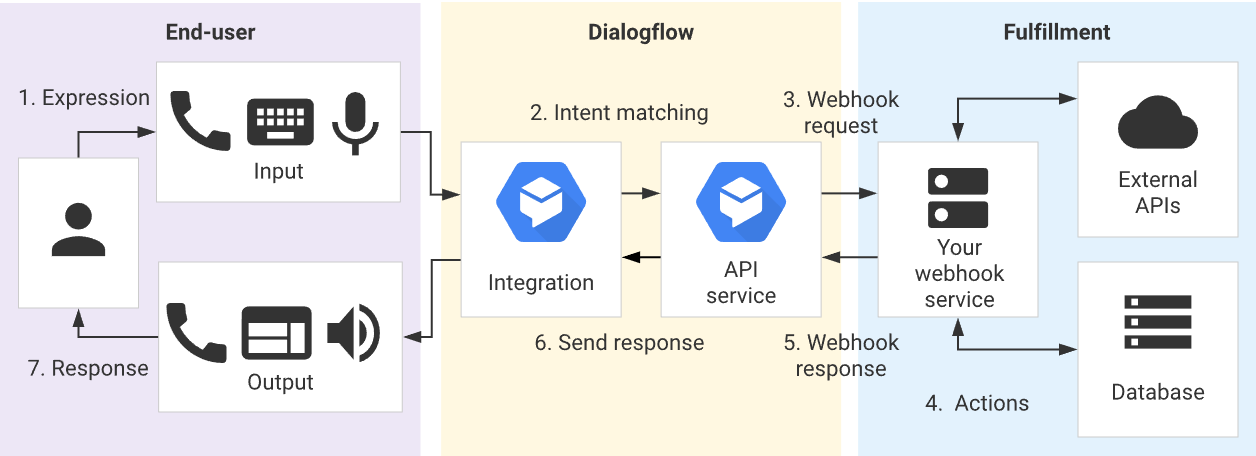
\includegraphics[width=1.0\textwidth]{fulfillment-flow}
    \caption{Flow-ul intern al Dialogflow \cite{google_dialogflow}.}
\end{figure}

În ansamblu, alegerea Dialogflow, împreună cu Google Cloud Functions, Google Source Repositories și Google Cloud Storage, oferă o soluție robustă și flexibilă pentru dezvoltarea de chatboti în sectorul bancar. Prin folosirea acestor tehnologii, băncile pot crea experiențe de conversație personalizate, eficiente și securizate pentru clienții lor.

\subsection{Cum funcționează ecosistemul}

Dialogflow folosește input-ul trimis de către Dialogflow API C++ Client \cite{dialogflow_client_library}, acesta fiind parsat și trecut prin verificarea lor internă cu intențiile create în prealabil\footnote{O intenție reprezintă un anumit rezultat pe care doriți să îl obțineți de la interacțiunea utilizatorului. De exemplu, o intenție poate fi „programare întâlnire” sau „informații despre cont”.}. În funcție de cum este creat intent-ul și scopul său, pot exista parametrii scoși sub formă de entități\footnote{Entitățile sunt concepte valoroase care pot fi extrase din declarațiile utilizatorilor. De exemplu, în declarația „Doresc să programez o întâlnire pentru marți”, „marți” este o entitate de tip „dată”.} din textul primit (sau este un intent default, cu rol de legătură între altele cu functionalități).

\begin{figure}[h]
    \centering
    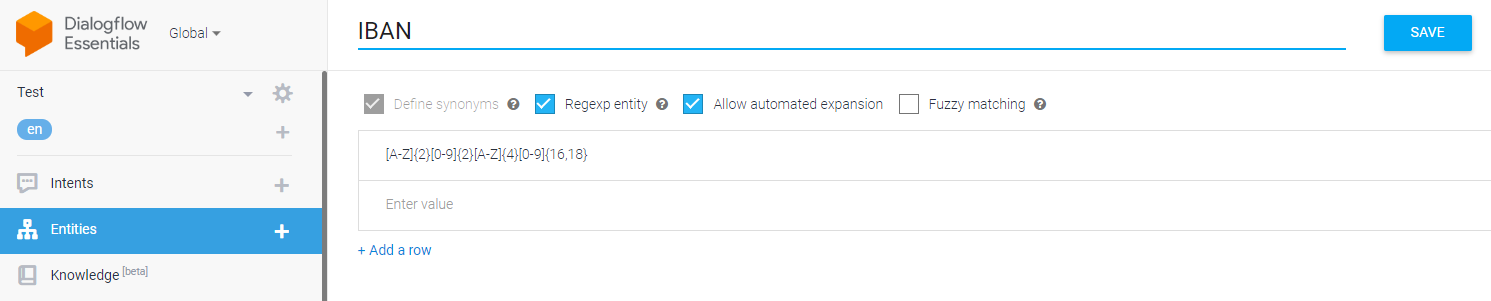
\includegraphics[width=1.0\textwidth]{entitati}
    \caption{Reprezentarea unei entități pentru IBAN folosind un regex.}
    \label{fig:entitati}
\end{figure}

În Dialogflow, o "intenție" reprezintă un anumit rezultat pe care îl doriți de la o interacțiune cu utilizatorul. Atunci când un utilizator trimite un input (cum ar fi o întrebare sau o comandă), Dialogflow potrivește inputul cu cea mai bună intenție pe baza a ceea ce ați setat în agentul dvs. În cadrul unei intenții, există mai multe câmpuri și concepte cheie care sunt utilizate pentru a defini și a rafina comportamentul intenției.

\textbf{Contextele} permit agentului Dialogflow să înțeleagă starea conversației și să răspundă în mod corespunzător. Există două tipuri de contexte: contexte de intrare și contexte de ieșire. Contextele de intrare sunt cele pe care agentul le caută înainte de a potrivi o intenție, în timp ce contextele de ieșire sunt stabilite după ce o intenție este potrivită.

\textbf{Exemple de declarații ale utilizatorului} sunt exemple de ceea ce utilizatorul ar putea spune pentru a declanșa această intenție (vezi Figura \ref{fig:training-phrases}). Sistemul utilizează aceste exemple pentru a învăța modelul de limbaj și pentru a recunoaște aceeași intenție din declarații diferite.

\begin{figure}[H]
    \centering
    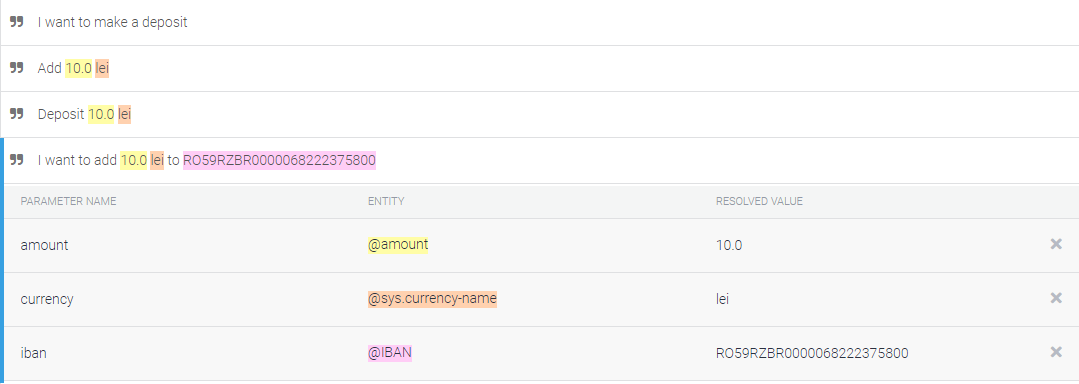
\includegraphics[width=1.0\textwidth]{training-phrases}
    \caption{Frazele de antrenament ale botului.}
    \label{fig:training-phrases}
\end{figure}

\textbf{Răspunsurile} reprezintă modul de interacționare hard-codată a agentului cu inputul clientului. Astfel, un răspuns toate fi considerat fie final de conversație, fie poate avea un răspuns default, folosind funcționalitatea webhook-ului ulterior.

\begin{figure}[H]
    \centering
    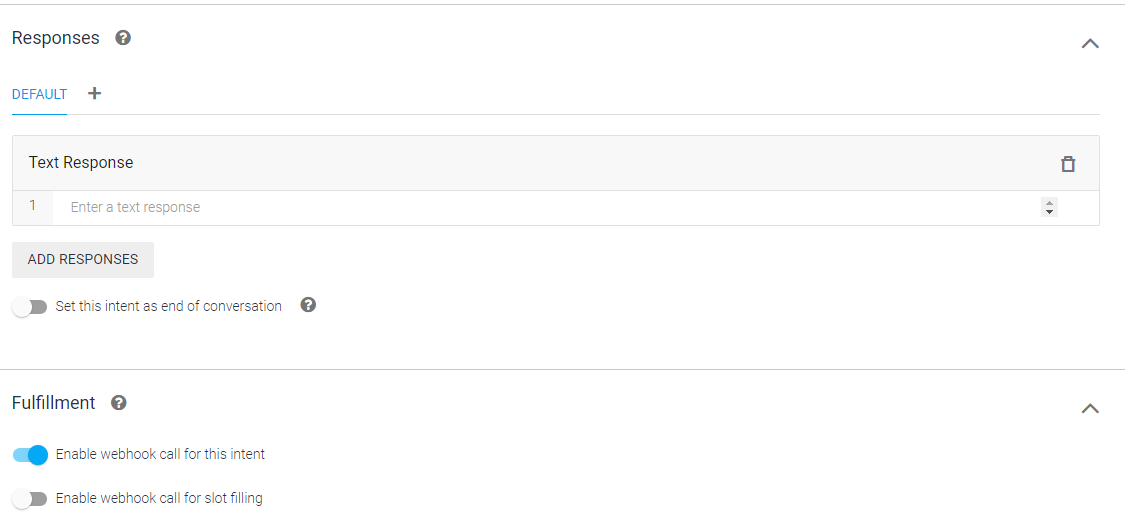
\includegraphics[width=1.0\textwidth]{fulfillment}
    \caption{Selectarea fulfillment-ului.}
    \label{fig:fulfillment}
\end{figure}

În cadrul platformei există niște entități predefinite \cite{system-entities} pentru a ușura munca utilizatorului atunci când vine vorba de extragere de parametrii, dar funcționalitatea puternică al acestei opțiuni este extragerea parametrizată a informațiilor. Dupa cum putea vedea in Figura \ref{fig:actiune-parametrii}, acțiunea propriu-zisă oferă flexibilitate atât la prezența parametrului (daca acesta se poate scoate din text), cât și la un text default dacă acesta nu a fost găsit. Coloana \emph{value} reprezintă numele variabilei care este trimisă către metoda din Google Cloud Function, prin webhook-ul definit în tabul de \emph{fulfillment}.

\begin{figure}[h]
    \centering
    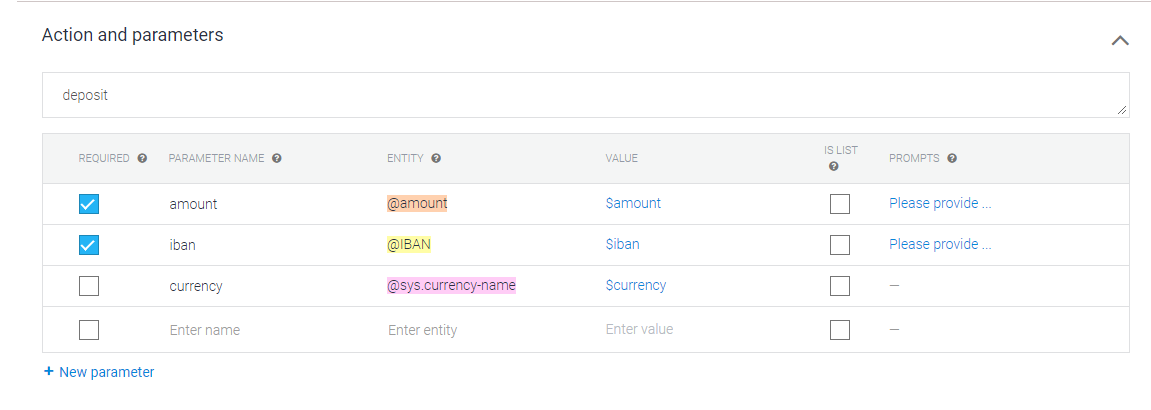
\includegraphics[width=1.0\textwidth]{actiune-parametrii}
    \caption{Extragerea de parametrii din inputul clientului.}
    \label{fig:actiune-parametrii}
\end{figure}

În tab-ul de fulfillment putem găsi modul de procesare al informației extrase de către agent. În cazul de față, am folosit un webhook extern, care folosește integrarea cu Google Cloud Function. Astfel, parametrii scoși vor fi trimiși sub forma unui request către acel URL. Detaliile acelui request se află în Figura \ref{fig:exemplu-request}.

\begin{figure}[h]
    \centering
    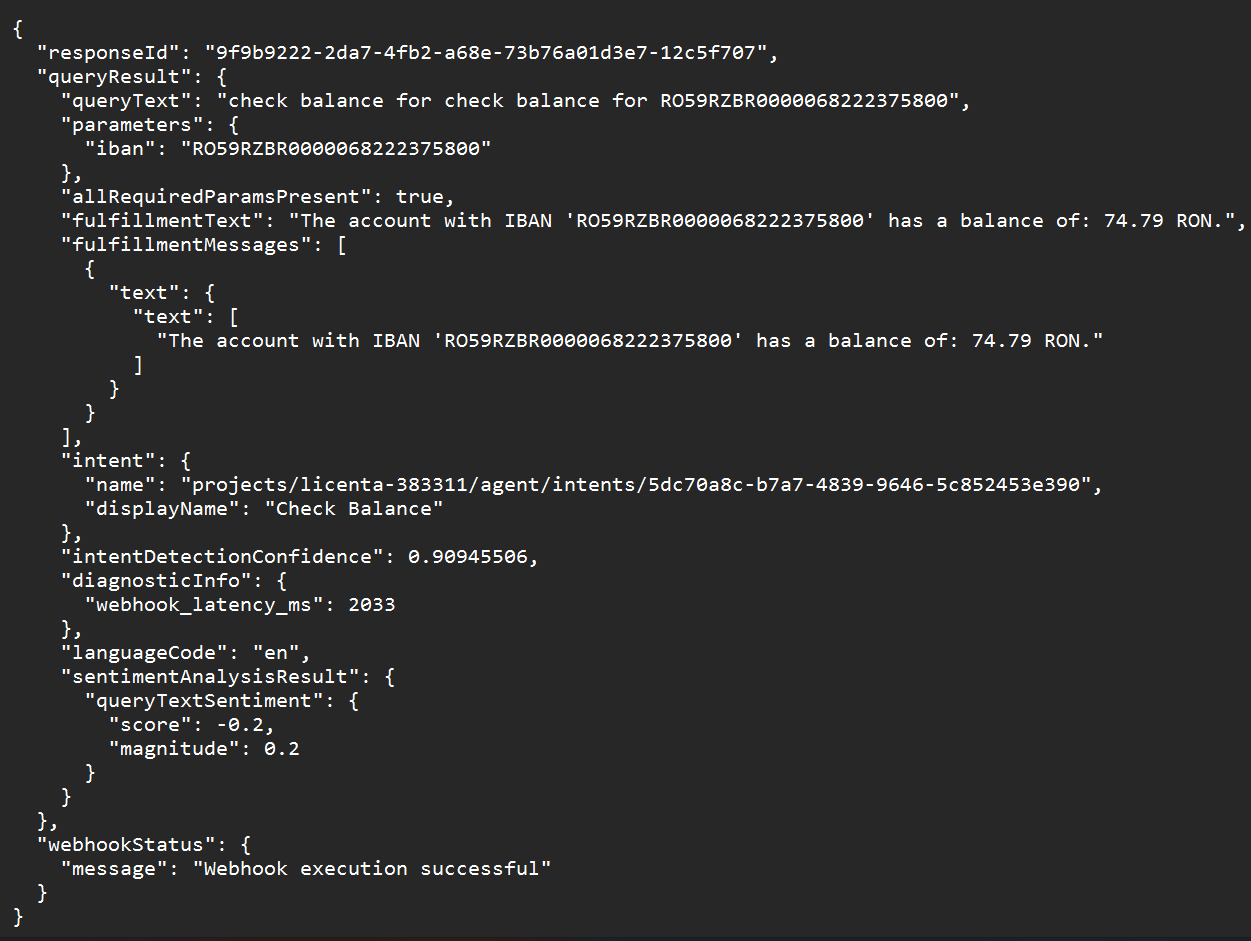
\includegraphics[width=1.0\textwidth]{exemplu-request}
    \caption{Exemplu de request trimis către Google Cloud Function.}
    \label{fig:exemplu-request}
\end{figure}

Explicațiile parametrului pentru o mai bună înțelegere a modului de transmitere a informației între seriviciile Google Cloud Platform:

\begin{enumerate}
    \item responseId: este un identificator unic pentru fiecare interacțiune cu Dialogflow.

    \item queryResult: este secțiunea care conține majoritatea informațiilor legate de interacțiunea cu utilizatorul.
    
    \subitem queryText: este întrebarea sau afirmația pe care utilizatorul a transmis-o.
    
    \subitem parameters: sunt parametrii extrasi din întrebarea utilizatorului. În acest caz, "iban" este un parametru și valoarea sa este "RO59RZBR0000068222375800".
    
    \subitem allRequiredParamsPresent: acest câmp indică dacă toți parametrii necesari pentru intenție sunt prezenți. În acest caz, este adevărat, ceea ce înseamnă că toți parametrii necesari sunt prezenți.
    
    \subitem fulfillmentText: este textul care va fi returnat utilizatorului ca răspuns la întrebarea sa.
    
    \subitem fulfillmentMessages: este o listă de mesaje care vor fi trimise înapoi utilizatorului. În acest caz, este doar un mesaj, care este același cu fulfillmentText.
    
    \subitem intent: este intenția care a fost potrivită pentru întrebarea utilizatorului.
    
    \subitem intentDetectionConfidence: este gradul de încredere cu care Dialogflow a potrivit intenția. În acest caz, este de aproximativ 90.
    
    \subitem diagnosticInfo: sunt informații suplimentare privind interacțiunea. În acest caz, indică timpul de latență pentru webhook.
    
    \subitem languageCode: este codul de limbă al interogării utilizatorului.
    
    \subitem sentimentAnalysisResult: este analiza sentimentului textului interogării. Scorul indică sentimentul general (pozitiv sau negativ), iar magnitudinea indică intensitatea sentimentului.
    
    \item webhookStatus: este statusul execuției webhook-ului, care în acest caz a fost reușită.
\end{enumerate}

Tabul de "Validation" din Dialogflow ES are de-a face cu revizuirea și aprobarea sau respingerea propunerilor pe care Dialogflow le face pentru îmbunătățirea modelului asistentului virtual. Acesta este un element al învățării automate interactive, unde sistemul învață din feedbackul dat de utilizator.

După ce asistentul virtual a fost folosit o vreme, va începe să învețe din interacțiunile cu utilizatorii și va încerca să îmbunătățească precizia detecției intențiilor și a entităților. Acest lucru este realizat prin generarea de "sugestii" pe baza interacțiunilor anterioare. Aceste sugestii apar în tabul "Validation".

Fiecare sugestie conține următoarele elemente:

Training phrase - Este textul interacțiunii dintre utilizator și asistentul virtual.

Intent - Este numele intenției pe care Dialogflow o propune pentru fraza de instruire. Acesta poate fi o intenție existentă sau o nouă intenție sugerată de Dialogflow.

Action - Este un câmp opțional, care permite asocierea unei acțiuni cu o intenție. Dialogflow poate sugera o acțiune pe baza contextului frazei de instruire.

Entities - Sunt entitățile pe care Dialogflow le propune pentru a fi asociate cu fraza de instruire.

Fiecare sugestie poate fi aprobată sau respinsă, în funcție de dorință (vezi Figura \ref{fig:validation}). Dacă sugestia este aprobată, Dialogflow va actualiza modelul asistentului virtual pentru a include informațiile din sugestie, îmbunătățind astfel precizia detecției de intenții și entități în interacțiunile viitoare. Dacă sugestia este respinsă, Dialogflow nu va face nicio modificare.

\begin{figure}[h]
    \centering
    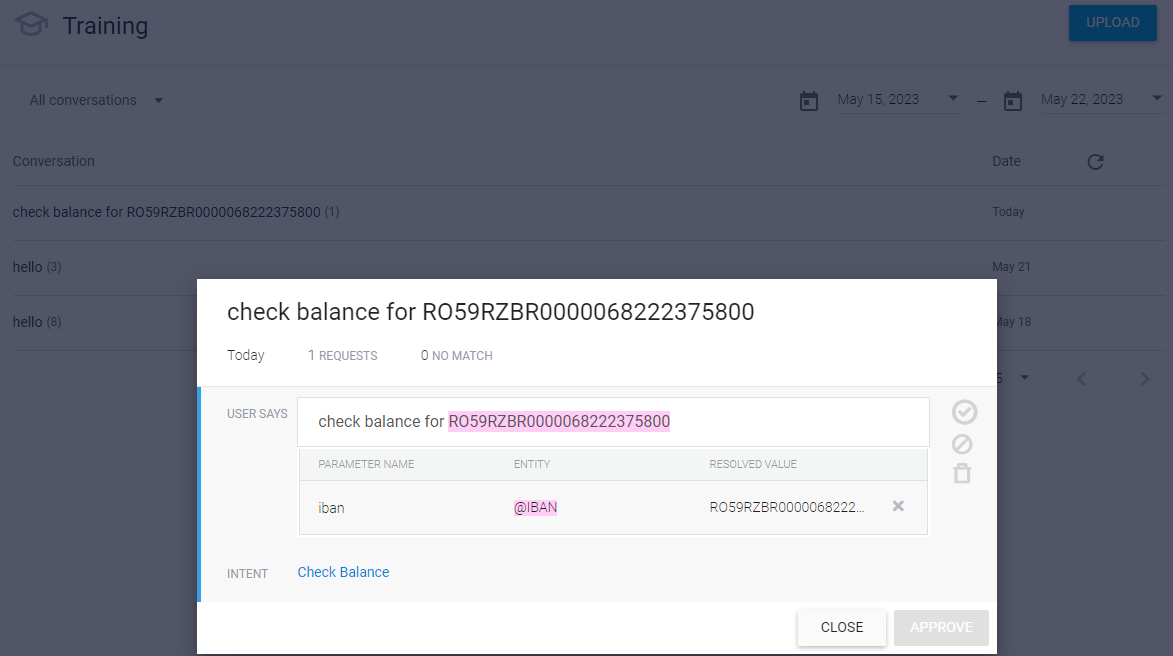
\includegraphics[width=1.0\textwidth]{validation}
    \caption{Validarea rezultatului agentului.}
    \label{fig:validation}
\end{figure}

\section{Alegerea utilitarului}

Biblioteca Portable Components (POCO) este un set popular de biblioteci open-source pentru dezvoltarea de software în C++. Se evidențiază printr-o gamă largă de facilități care îi permit să fie o soluție potrivită pentru dezvoltarea unei aplicații web. Înainte de a trece la detaliile bibliotecii POCO, este esențial să se înțeleagă contextul general al instrumentelor și bibliotecilor disponibile pentru dezvoltarea aplicațiilor web în C++.

Din punct de vedere istoric, dezvoltarea aplicațiilor web în C++ a fost deseori privită ca un proces complex, în mare parte din cauza faptului că limbajul C++ este orientat spre dezvoltarea software de nivel înalt, cu un control detaliat asupra resurselor hardware, precum și a complexității implicite a acestui limbaj. Cu toate acestea, cu ajutorul unor instrumente precum bibliotecile POCO \cite{poco-docs}, Boost \cite{boost-docs}, Wt \cite{wt-docs} și CPPCMS \cite{cppcms-docs}, dezvoltarea aplicațiilor web în C++ a devenit mult mai ușoară și mai eficientă.

\subsection{POCO: avantaje și caracteristici}

POCO se distinge prin designul său robust și portabil, care permite dezvoltatorilor să creeze software eficient și de înaltă performanță, care poate fi portat cu ușurință pe diferite platforme și sisteme de operare. Bibliotecile POCO au fost concepute pentru a fi ușor de înțeles și de utilizat, fără a impune niciun model de programare specific. Acest lucru le face flexibile și adaptabile, încurajând dezvoltarea rapidă și agile.

În contextul dezvoltării aplicațiilor web, biblioteca POCO oferă numeroase facilități, inclusiv suport pentru HTTP, FTP, sendmail, URI, cookie-uri, HTML formular și altele. Acesta include, de asemenea, un framework pentru servere web, care permite dezvoltarea serverelor web multithreaded și sigure. De asemenea, biblioteca NetSSL furnizează suport pentru comunicațiile securizate SSL/TLS, care sunt esențiale pentru orice aplicație web modernă.

\subsection{POCO în comparație cu alte biblioteci C++}

Să comparăm acum POCO cu alte biblioteci C++ populare pentru dezvoltarea aplicațiilor web: Boost, Wt și CPPCMS.

Boost este o colecție vastă de biblioteci C++, care oferă o gamă largă de facilități. Cu toate acestea, Boost nu este specializat în dezvoltarea aplicațiilor web și nu include suport direct pentru HTTP sau alte protocoale web specifice. Prin urmare, dezvoltarea unei aplicații web cu Boost ar necesita o cantitate semnificativă de cod adițional sau utilizarea altor biblioteci pentru a acoperi aceste funcționalități.

Wt este o bibliotecă C++ pentru dezvoltarea aplicațiilor web care utilizează un model de programare similar cu cel al Qt. Deși Wt este puternic și flexibil, are un model de programare mai complex decât POCO și poate fi mai dificil de învățat și de utilizat, în special pentru cei care nu sunt familiarizați cu Qt.

CPPCMS este un framework specializat pentru dezvoltarea aplicațiilor web în C++. Deși CPPCMS include o serie de facilități puternice pentru dezvoltarea aplicațiilor web, el impune un anumit model de programare, care poate fi mai restrictiv decât abordarea mai flexibilă a POCO.

Prin urmare, POCO oferă un echilibru excelent între ușurința de utilizare, flexibilitate, portabilitate și performanță, ceea ce o face o alegere bună pentru dezvoltarea aplicațiilor web în C++. Cu toate acestea, alegerea finală ar trebui să depindă de cerințele specifice ale proiectului, de preferințele dezvoltatorului și de alte considerații.